\documentclass{article}

\PassOptionsToPackage{numbers,sort&compress}{natbib}
\usepackage[preprint]{neurips}
\usepackage[utf8]{inputenc}
\usepackage[T1]{fontenc}
\usepackage{hyperref}
\usepackage{url}
\usepackage{booktabs}
\usepackage{amsfonts}
\usepackage{nicefrac}
\usepackage{microtype}
\usepackage{xcolor}
\usepackage{graphicx}
\usepackage{subcaption}
\usepackage{multirow}
\usepackage{array}
\usepackage{float}
\usepackage{adjustbox}
\usepackage{amsthm}
\usepackage{amsmath}
\usepackage{amssymb}
\usepackage{mathtools}
\usepackage{enumitem}
\usepackage{algorithm}
\usepackage{algpseudocode}
\usepackage{bbm}

\title{TRIBE: Post-hoc Domain Generalization by Trajectory-Induced Basis Editing}
\author{Anonymous Authors}

\newtheorem{theorem}{Theorem}
\newtheorem{proposition}{Proposition}
\newtheorem{lemma}{Lemma}
\newtheorem{corollary}{Corollary}
\newtheorem{definition}{Definition}
\newtheorem{assumption}{Assumption}
\newtheorem{remark}{Remark}

\newcommand{\RR}{\mathbb{R}}
\newcommand{\EE}{\mathbb{E}}
\newcommand{\PP}{\mathbb{P}}
\newcommand{\cA}{\mathcal{A}}
\newcommand{\cB}{\mathcal{B}}
\newcommand{\cD}{\mathcal{D}}
\newcommand{\cF}{\mathcal{F}}
\newcommand{\cH}{\mathcal{H}}
\newcommand{\cQ}{\mathcal{Q}}
\newcommand{\cR}{\mathcal{R}}
\newcommand{\cS}{\mathcal{S}}
\newcommand{\cT}{\mathcal{T}}
\newcommand{\cU}{\mathcal{U}}
\newcommand{\cV}{\mathcal{V}}
\newcommand{\cW}{\mathcal{W}}
\newcommand{\cX}{\mathcal{X}}
\newcommand{\argmin}{\operatorname*{arg\,min}}
\newcommand{\argmax}{\operatorname*{arg\,max}}
\newcommand{\rank}{\operatorname{rank}}
\newcommand{\spanop}{\operatorname{span}}
\newcommand{\simplex}{\Delta}
\newcommand{\diag}{\operatorname{diag}}
\newcommand{\tr}{\operatorname{tr}}
\newcommand{\softmax}{\operatorname{softmax}}
\newcommand{\TBD}{\textbf{TBD}}
\newcommand{\tribe}{\textup{\textsc{TRIBE}}}
\newcommand{\swad}{\textup{\textsc{SWAD}}}
\newcommand{\diwa}{\textup{\textsc{DiWA}}}
\newcommand{\miro}{\textup{\textsc{MIRO}}}
\newcommand{\erm}{\textup{\textsc{ERM}}}
\newcommand{\ood}{OOD}
\newcommand{\iid}{i.i.d.}
\newcommand{\1}{\mathbbm{1}}
\newcommand{\abs}[1]{\left\lvert #1 \right\rvert}
\newcommand{\norm}[1]{\left\lVert #1 \right\rVert}
\newcommand{\paren}[1]{\left( #1 \right)}
\newcommand{\bracks}[1]{\left[ #1 \right]}
\newcommand{\braces}[1]{\left\{ #1 \right\}}
\newcommand{\loss}{\ell}
\newcommand{\inner}[2]{\left\langle #1, #2 \right\rangle}

\begin{document}

\maketitle

\begin{abstract}
Single-run post-hoc domain generalization has become attractive because it can be attached to a strong empirical-risk-minimization pipeline without retraining the full network. The strongest deployed methods in this regime typically average checkpoints from a dense trajectory, using flatness, connectivity, or validation heuristics to define the final predictor. This paper studies a different remaining degree of freedom: once a strong post-hoc anchor has already been selected, can one perform a small, domain-label-free correction of the classifier boundary itself? We propose \textbf{\tribe{}} (\textbf{Tr}ajectory-\textbf{I}nduced \textbf{B}asis \textbf{E}diting), a post-hoc method that first fixes an averaged anchor from one dense run, then extracts low-rank failure modes from checkpoint-response trajectories on a pooled source holdout, and finally performs a local robust last-layer repair against worst-case mixtures of those trajectory modes. The method is explicitly domain-label-free, deploys a single model, and keeps the representation fixed during the repair stage. We prove strong convexity and uniqueness of the repair objective, a minimax characterization of the induced low-rank uncertainty family, a monotone empirical certificate relative to the fixed anchor, a spectral perturbation result for recovery of trajectory modes under a spiked response model, and a conditional target-risk certificate under source-supported head-repairable shift. The experimental sections intentionally leave new \tribe{} results as \TBD{}, while recording the exact evaluation protocol and published benchmark context from prior work.
\end{abstract}

\section{Introduction}

Domain generalization (DG) asks for a predictor that performs well on an unseen target environment using only source data during training. In practice, the DG methods that persist are often the ones that do not require retraining everything from scratch. Post-hoc selectors are therefore especially attractive: train once, save dense checkpoints, and then choose one deployable predictor after training has already finished.

This design space already contains strong ideas. Interval-based flat-minima selectors improved average out-of-domain accuracy on the standard DomainBed benchmark family from \(63.3\) to \(66.9\) without changing the base training algorithm \citep{cha2021swad}. Pretraining-aware DG combined with the same post-hoc selection logic reaches \(68.1\) on the same benchmark family \citep{cha2022miro}. Weight averaging and model soups established a broader lesson: the final predictor is often not the last checkpoint, and averaging can help when the models remain in a connected low-loss region \citep{izmailov2018swa,frankle2020linear,wortsman2022soups,rame2022diwa}.

Still, there is a visible ceiling. Existing single-run post-hoc DG methods almost all operate inside one action family: \emph{pick or average checkpoints}. They can move the deployed predictor to a flatter region, a safer interval, or a better soup, but they cannot directly repair a residual decision-boundary error once the representation is already good. That limitation matters if the remaining target error is not primarily a basin-selection problem but a \emph{minority-feature underweighting problem} in the final classifier layer.

This paper studies that missing degree of freedom. We propose \textbf{\tribe{}} (\textbf{Tr}ajectory-\textbf{I}nduced \textbf{B}asis \textbf{E}diting), a post-hoc, domain-label-free DG method with two stages:
\begin{enumerate}[leftmargin=1.4em]
    \item fix a strong averaged \emph{anchor} model from the dense checkpoint bank, and
    \item perform a \emph{local robust last-layer repair} using a low-rank basis extracted from how source examples behave across the checkpoint trajectory.
\end{enumerate}

The central object is a \emph{trajectory response matrix}. For each held-out source example and each checkpoint, we record a response statistic such as signed margin or loss relative to the anchor. Examples whose responses co-vary across checkpoints reveal latent failure directions that do not require domain labels. A low-rank basis of that response matrix defines a structured uncertainty family over hidden source-supported shifts. \tribe{} then repairs only the last layer of the fixed anchor by minimizing the worst-case loss over that uncertainty family, subject to a locality penalty that keeps the repaired head close to the anchor.

The resulting method is motivated by three observations from adjacent theory.
\begin{itemize}[leftmargin=1.4em]
    \item Flat minima are useful because they control a robust empirical-risk object over neighborhoods in parameter space \citep{cha2021swad}.
    \item Weight averaging under shift depends on diversity and locality jointly, not on flatness alone \citep{rame2022diwa}.
    \item Last-layer retraining can substantially improve subgroup robustness even without group labels, especially when one can construct a better reweighting set or feature weighting after the base model is fixed \citep{qiu2023afr,labonte2023self,roburin2023gram}.
\end{itemize}
These lines suggest a concrete hypothesis:
\begin{quote}
\textbf{After a strong averaged anchor is fixed, part of the remaining DG error can be removed by a small, local classifier-head correction targeted at trajectory-stable hidden failure directions.}
\end{quote}

The paper does \emph{not} claim an unconditional theorem that \tribe{} empirically dominates every flat-minima selector, soup rule, or robust classifier baseline. That would be indefensible. The strongest honest claim is narrower and more useful: under explicit assumptions, \tribe{} directly optimizes a robust local-repair objective over the deployed model class itself, and it can be shown to improve a worst-case certificate relative to the fixed anchor whenever the remaining shift is source-supported and head-repairable.

Our contributions are:
\begin{enumerate}[leftmargin=1.4em]
    \item We introduce \tribe{}, a domain-label-free, single-run post-hoc DG method that combines a fixed averaged anchor with trajectory-induced local robust head repair.
    \item We define a low-rank trajectory-failure basis and the corresponding uncertainty family over hidden source-supported shifts.
    \item We prove strong convexity, uniqueness, a saddle-point characterization, and standard convergence guarantees for the repair stage.
    \item We prove a monotone empirical certificate relative to the fixed anchor, a spectral recovery result for the trajectory basis under a spiked response model, and a conditional target-risk certificate under head-repairable shift.
    \item We provide a full experimental protocol, published benchmark context from prior DG work, and \TBD{} placeholders for the new \tribe{} experiments.
\end{enumerate}

\begin{figure}[t]
    \centering
    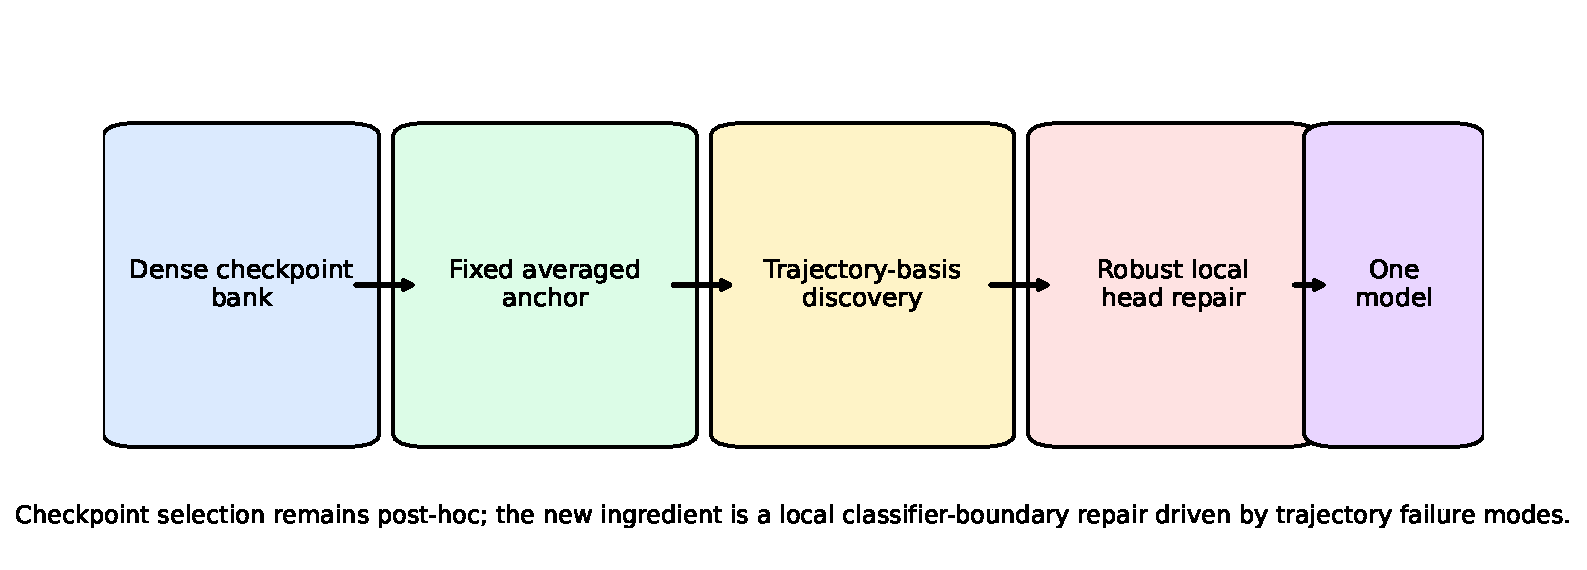
\includegraphics[width=\linewidth]{figures/tribe_overview.pdf}
    \caption{\textbf{\tribe{} overview.} A dense checkpoint bank first yields a fixed averaged anchor on a dedicated source split. On a separate discovery split, checkpoint-response trajectories are factorized into a low-rank failure basis. On a repair split, the basis induces a domain-label-free uncertainty family over hidden source-supported shifts, and a local last-layer repair is solved around the fixed anchor.}
    \label{fig:overview}
\end{figure}

\section{Related Work}

\paragraph{Single-run post-hoc DG.}
Flat-minima interval selectors showed that strong DG gains can be obtained by changing only the post-hoc selection rule, not the training algorithm \citep{cha2021swad}. Their success is one of the main motivations for this paper: single-run, one-model test-time methods are operationally valuable. \tribe{} keeps that regime, but it adds one degree of freedom beyond checkpoint selection: a local head repair around a fixed anchor.

\paragraph{Weight averaging, soups, and locality.}
Stochastic weight averaging, mode connectivity, and model soups established that averaging nearby models can improve generalization when they lie in a connected low-loss basin \citep{izmailov2018swa,garipov2018fge,frankle2020linear,wortsman2022soups}. \diwa{} clarified the \ood{} picture by deriving a bias--variance--covariance--locality decomposition and emphasizing that diversity and locality must be traded off rather than optimized independently \citep{rame2022diwa}. \tribe{} preserves that lesson by using a fixed averaged anchor and restricting the repair to a local neighborhood around its classifier head.

\paragraph{Subpopulation robustness without group labels.}
Hidden-subpopulation shift and worst-group robustness have motivated distributionally robust and fairness-aware learning without explicit demographics \citep{hashimoto2018fairness,sagawa2020groupdro,li2021worstcase,yang2023change}. Recent methods show that robustness can be improved by post-hoc reweighting or last-layer retraining without full group annotations \citep{qiu2023afr,labonte2023self,roburin2023gram}. \tribe{} belongs to this family in spirit, but its discovery signal is specific to post-hoc single-run DG: the geometry of checkpoint-response trajectories.

\paragraph{Why trajectory geometry matters.}
Most no-group-label robustness methods discover hard examples from feature statistics, misclassifications, or disagreement between separately chosen models. \tribe{} instead uses a source of structure unique to dense post-hoc replay: how each example's margin and loss evolve across a checkpoint bank. This creates a new kind of latent object, a \emph{trajectory failure mode}, that does not exist in ordinary single-model group-robust pipelines.

\section{Problem Setup}
\label{sec:setup}

We consider multiclass classification with a dense checkpoint bank
\[
    \{\theta_t\}_{t=1}^{T},
\]
produced by a single training run. Each checkpoint decomposes into a feature map and classifier head,
\[
    \theta_t = (\phi_t, W_t),
\]
where \(W_t \in \RR^{d\times C}\) maps \(d\)-dimensional features to \(C\) logits.

Post-hoc processing uses four disjoint pooled source holdout splits:
\begin{itemize}[leftmargin=1.4em]
    \item \(\cD_{\mathrm{sel}}\): anchor selection,
    \item \(\cD_{\mathrm{basis}}\): trajectory-basis discovery,
    \item \(\cD_{\mathrm{repair}}\): head repair,
    \item \(\cD_{\mathrm{val}}\): model selection.
\end{itemize}
These sets are pooled across source domains and do not use source-domain identities.

\subsection{Stage 1: Fixed averaged anchor}

Let \(\cA\) denote a family of domain-label-free post-hoc anchor rules. An element \(A\in\cA\) may be a single checkpoint, a contiguous interval average, or a soup over a preselected subset of checkpoints. The theory in this paper is \emph{conditional} on the returned anchor; it does not require one specific anchor-selection algorithm.

\begin{definition}[Fixed deployed anchor]
A fixed deployed anchor is a model
\[
    A = (\phi_A, W_0)
\]
selected using only \(\cD_{\mathrm{sel}}\), and then frozen before basis discovery, head repair, and validation.
\end{definition}

The important point is not whether the anchor is a single checkpoint or an average, but that it is chosen first and then treated as fixed throughout the rest of the pipeline. In practice, the most natural anchor is an averaged model because averaging already improves DG in prior work \citep{cha2021swad,wortsman2022soups,rame2022diwa}. The theory accommodates either choice.

\subsection{Stage 2: Trajectory response matrix}

For any labeled example \((x,y)\), define the true-class signed margin of checkpoint \(t\) by
\begin{equation}
    m_t(x,y)
    \triangleq
    f_t(x)_y - \max_{c\neq y} f_t(x)_c,
    \label{eq:margin}
\end{equation}
where \(f_t(x)=W_t^\top \phi_t(x)\) are the checkpoint logits. The anchor margin is \(m_A(x,y)\).

On \(\cD_{\mathrm{basis}} = \{(x_i,y_i)\}_{i=1}^{n_B}\), define the trajectory-response residual matrix \(R\in\RR^{n_B\times T}\) by
\begin{equation}
    R_{it}
    \triangleq
    m_t(x_i,y_i) - m_A(x_i,y_i).
    \label{eq:trajectory_matrix}
\end{equation}
Let \(H_n = I_n - \frac{1}{n}\1\1^\top\) denote the centering matrix. We center the response matrix along the example and checkpoint axes:
\begin{equation}
    \widetilde R
    \triangleq
    H_{n_B} \, R \, H_T.
    \label{eq:centered_matrix}
\end{equation}
Its truncated singular value decomposition is
\begin{equation}
    \widetilde R \approx \widehat U_k \widehat \Sigma_k \widehat V_k^\top,
    \label{eq:svd}
\end{equation}
where \(\widehat V_k \in \RR^{T\times k}\) collects the top \(k\) right singular vectors.

\begin{definition}[Trajectory failure basis]
The matrix \(\widehat V_k\) is the trajectory failure basis. For any example \((x,y)\), define its centered trajectory vector
\begin{equation}
    \widetilde r(x,y)
    \triangleq
    \paren{m_1(x,y)-m_A(x,y), \dots, m_T(x,y)-m_A(x,y)} H_T
    \in \RR^{T},
    \label{eq:trajectory_vector}
\end{equation}
and its trajectory-basis coordinates
\begin{equation}
    z(x,y)
    \triangleq
    \widetilde r(x,y)\,\widehat V_k
    \in \RR^k.
    \label{eq:basis_score}
\end{equation}
\end{definition}

The role of \(\widehat V_k\) is not to recover semantic classes or true latent domains. It is only to extract low-rank directions along which held-out source examples show correlated margin instability across the checkpoint bank.

\begin{figure}[t]
    \centering
    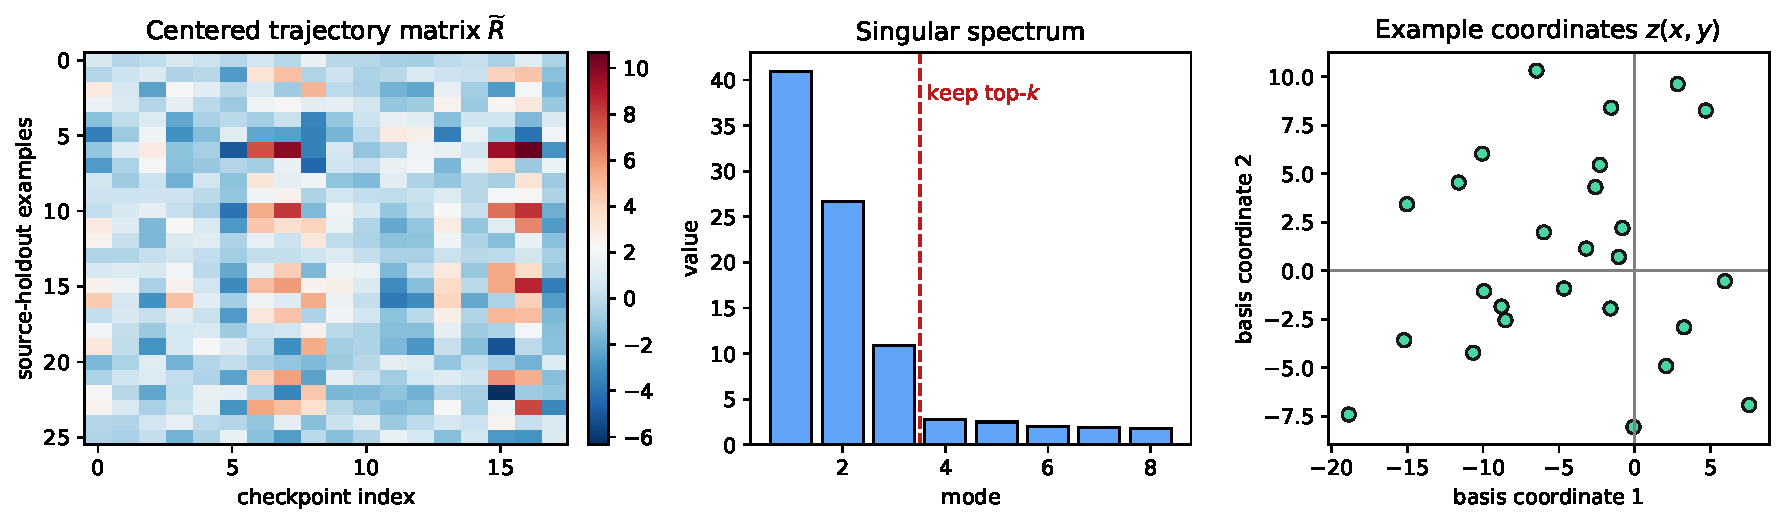
\includegraphics[width=\linewidth]{figures/trajectory_basis_pipeline.pdf}
    \caption{\textbf{Trajectory basis construction.} Example-by-checkpoint margin residuals are centered and factorized. The right singular directions define checkpoint-space failure modes; any new example is mapped to a low-dimensional trajectory coordinate by projection onto those modes.}
    \label{fig:basis}
\end{figure}

\subsection{Stage 3: Basis-induced uncertainty set}

On the repair split \(\cD_{\mathrm{repair}}=\{(x_i,y_i)\}_{i=1}^{n_R}\), compute the basis-score matrix
\begin{equation}
    Z
    \triangleq
    \begin{bmatrix}
        z(x_1,y_1)^\top \\
        \vdots \\
        z(x_{n_R},y_{n_R})^\top
    \end{bmatrix}
    \in \RR^{n_R\times k},
    \qquad
    \1^\top Z = 0,
    \label{eq:score_matrix}
\end{equation}
where the last identity follows from centering.

Let \(u_{n_R}=\frac{1}{n_R}\1\) denote the uniform distribution on \(\cD_{\mathrm{repair}}\). The basis-induced uncertainty family is
\begin{equation}
    \cQ_\rho(Z)
    \triangleq
    \braces{
        q \in \simplex^{n_R-1} :
        q = u_{n_R} + Z\beta,\;
        \norm{\beta}_2 \le \rho
    }.
    \label{eq:q_family}
\end{equation}
This set contains only source-supported shifts and allows the adversary to move mass along the discovered trajectory directions, but only within a low-dimensional radius-\(\rho\) cone.

\begin{remark}
The construction in Eq.~\eqref{eq:q_family} deliberately avoids hard pseudo-group assignments. The adversary moves continuously in the low-rank trajectory subspace rather than over an explicit clustering of examples into latent groups.
\end{remark}

\subsection{Stage 4: Local head repair}

The repaired model keeps the anchor feature map \(\phi_A\) fixed. Only the classifier head moves. For \(x\in\cX\), define anchor features \(\phi_A(x)\in\RR^d\).

The local repair class is
\begin{equation}
    \cW_r(W_0)
    \triangleq
    \braces{
        W \in \RR^{d\times C} :
        \norm{W-W_0}_F \le r
    }.
    \label{eq:local_class}
\end{equation}
The per-example cross-entropy loss is
\begin{equation}
    \loss_i(W)
    \triangleq
    - \log \frac{\exp\bracks{\inner{W_{:,y_i}}{\phi_A(x_i)}}}{\sum_{c=1}^C \exp\bracks{\inner{W_{:,c}}{\phi_A(x_i)}}}.
    \label{eq:ce_loss}
\end{equation}

\tribe{} solves the robust local head-repair problem
\begin{equation}
    \widehat W
    \in
    \argmin_{W \in \cW_r(W_0)}
    \sup_{q\in\cQ_\rho(Z)}
    \sum_{i=1}^{n_R} q_i \loss_i(W)
    +
    \frac{\lambda}{2}\norm{W-W_0}_F^2.
    \label{eq:tribe_objective}
\end{equation}
The deployed predictor is the single repaired model
\[
    \widehat \theta_{\mathrm{TRIBE}} = (\phi_A,\widehat W).
\]

\begin{remark}
Eq.~\eqref{eq:tribe_objective} optimizes the deployed object directly. There is no predictive-mixture bridge and no second-stage relaxation that differs from the final model sent to test time.
\end{remark}

\begin{figure}[t]
    \centering
    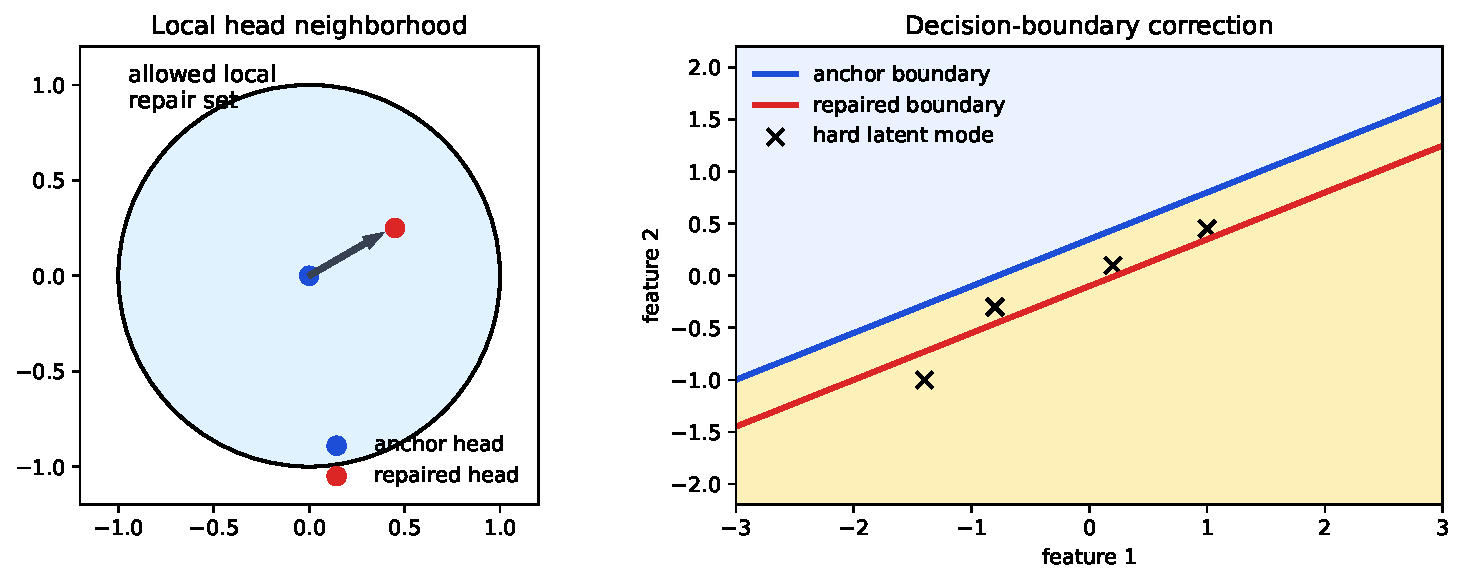
\includegraphics[width=\linewidth]{figures/local_repair_geometry.pdf}
    \caption{\textbf{Local head repair around a fixed averaged anchor.} The anchor head \(W_0\) defines a local ball in classifier space. Robust optimization moves only inside this neighborhood, preserving the anchor representation while correcting boundary error along trajectory-induced shift directions.}
    \label{fig:repair}
\end{figure}

\section{Theoretical Analysis}
\label{sec:theory}

This section states the main theorem package. All proofs appear in the appendix.

\subsection{Basic assumptions}

\begin{assumption}[Bounded anchor features]
\label{ass:bounded_features}
There exists \(R_\phi > 0\) such that
\[
    \norm{\phi_A(x)}_2 \le R_\phi
    \qquad \text{for all } x \text{ in the support of the source holdout.}
\]
\end{assumption}

\begin{assumption}[Interior feasibility of the uncertainty family]
\label{ass:interior_q}
The radius \(\rho\) is chosen so that \(\cQ_\rho(Z)\) is nonempty and compact.
\end{assumption}

\begin{assumption}[Spiked trajectory model]
\label{ass:spiked}
The centered trajectory matrix on \(\cD_{\mathrm{basis}}\) obeys
\[
    \widetilde R = M_\star + E,
    \qquad
    \rank(M_\star)=k,
\]
where \(M_\star\) has singular gap
\[
    \sigma_k(M_\star) - \sigma_{k+1}(M_\star) = \gamma_\star > 0,
\]
and \(E\) is a perturbation matrix with bounded operator norm.
\end{assumption}

\begin{assumption}[Source-supported head-repairable shift]
\label{ass:head_repairable}
The target distribution can be written as a reweighting of the source-support repair split:
\[
    R_T(W) = \sum_{i=1}^{n_R} q_i^\star \loss_i(W)
\]
for some \(q^\star \in \cQ_\rho(Z_\star)\), where \(Z_\star\) is the score matrix generated by the population trajectory basis. Moreover, there exists \(W^\dagger \in \cW_r(W_0)\) such that
\[
    \sup_{q\in\cQ_\rho(Z_\star)} R_q(W^\dagger)
    \le
    \sup_{q\in\cQ_\rho(Z_\star)} R_q(W_0) - \Delta
\]
for some \(\Delta>0\).
\end{assumption}

Assumption~\ref{ass:head_repairable} is the key modeling assumption of \tribe{}. It does not say that all DG shifts are head-repairable. It says only that if the remaining target shift after fixing a strong anchor is predominantly a classifier-boundary problem and is visible in the trajectory basis, then robust local repair is the right action.

\subsection{Convexity, saddle structure, and convergence}

\begin{proposition}[Convexity and uniqueness]
\label{prop:convexity}
Under Assumptions~\ref{ass:bounded_features} and \ref{ass:interior_q}, the map
\[
    \widehat J(W)
    \triangleq
    \sup_{q\in\cQ_\rho(Z)}
    \sum_{i=1}^{n_R} q_i \loss_i(W)
    +
    \frac{\lambda}{2}\norm{W-W_0}_F^2
\]
is \(\lambda\)-strongly convex on \(\cW_r(W_0)\). Consequently, the minimizer \(\widehat W\) in Eq.~\eqref{eq:tribe_objective} exists and is unique.
\end{proposition}

\begin{proposition}[Saddle-point formulation]
\label{prop:saddle}
Define
\[
    \widehat{\mathcal L}(W,q)
    \triangleq
    \sum_{i=1}^{n_R} q_i \loss_i(W)
    +
    \frac{\lambda}{2}\norm{W-W_0}_F^2.
\]
Then \(\widehat{\mathcal L}\) is convex in \(W\), linear in \(q\), and admits a saddle point on \(\cW_r(W_0)\times \cQ_\rho(Z)\):
\[
    \min_{W\in\cW_r(W_0)} \max_{q\in\cQ_\rho(Z)} \widehat{\mathcal L}(W,q)
    =
    \max_{q\in\cQ_\rho(Z)} \min_{W\in\cW_r(W_0)} \widehat{\mathcal L}(W,q).
\]
\end{proposition}

\begin{theorem}[Projected primal--dual convergence]
\label{thm:convergence}
Assume additionally that projected subgradients of \(\widehat{\mathcal L}\) are bounded by \(G\) on \(\cW_r(W_0)\times \cQ_\rho(Z)\), and let \(D_W,D_Q\) denote the diameters of the two feasible sets. Then projected primal--dual subgradient iterates with step size
\[
    \eta_t = \frac{\sqrt{D_W^2 + D_Q^2}}{G\sqrt{t}}
\]
produce averaged iterates \((\bar W_T,\bar q_T)\) with saddle residual
\[
    \max_{q\in\cQ_\rho(Z)} \widehat{\mathcal L}(\bar W_T,q)
    -
    \min_{W\in\cW_r(W_0)} \widehat{\mathcal L}(W,\bar q_T)
    \le
    \frac{2G\sqrt{D_W^2+D_Q^2}}{\sqrt{T}}.
\]
\end{theorem}

\subsection{Monotone certificate relative to the anchor}

\begin{theorem}[Anchor domination on the robust surrogate]
\label{thm:anchor_domination}
Let \(\widehat W\) solve Eq.~\eqref{eq:tribe_objective}. Since \(W_0 \in \cW_r(W_0)\), we have
\[
    \widehat J(\widehat W) \le \widehat J(W_0).
\]
Equivalently,
\[
    \sup_{q\in\cQ_\rho(Z)} \sum_{i=1}^{n_R} q_i \loss_i(\widehat W)
    +
    \frac{\lambda}{2}\norm{\widehat W-W_0}_F^2
    \le
    \sup_{q\in\cQ_\rho(Z)} \sum_{i=1}^{n_R} q_i \loss_i(W_0).
\]
\end{theorem}

This theorem is intentionally modest. It does not say the repaired model is universally better than the anchor on every possible target domain. It says that, on the robust surrogate \tribe{} explicitly chooses to defend against, the repaired head cannot be worse than leaving the anchor unchanged.

\subsection{A closed-form view of the adversary}

\begin{proposition}[Support-function form]
\label{prop:support}
Suppose the positivity constraint in Eq.~\eqref{eq:q_family} is inactive on the radius-\(\rho\) set, so that
\[
    \cQ_\rho(Z)
    =
    \braces{
        u_{n_R} + Z\beta : \norm{\beta}_2 \le \rho
    }.
\]
Then for any vector \(a\in\RR^{n_R}\),
\[
    \sup_{q\in\cQ_\rho(Z)} \inner{q}{a}
    =
    \frac{1}{n_R}\sum_{i=1}^{n_R} a_i
    +
    \rho \norm{Z^\top a}_2.
\]
In particular,
\[
    \widehat J(W)
    =
    \frac{1}{n_R}\sum_{i=1}^{n_R}\loss_i(W)
    +
    \rho \norm{Z^\top \loss(W)}_2
    +
    \frac{\lambda}{2}\norm{W-W_0}_F^2,
\]
where \(\loss(W) = (\loss_1(W),\dots,\loss_{n_R}(W))^\top\).
\end{proposition}

Proposition~\ref{prop:support} reveals the geometry of \tribe{}: it minimizes mean repair loss plus a penalty on the component of the loss vector aligned with the discovered trajectory failure basis.

\begin{figure}[t]
    \centering
    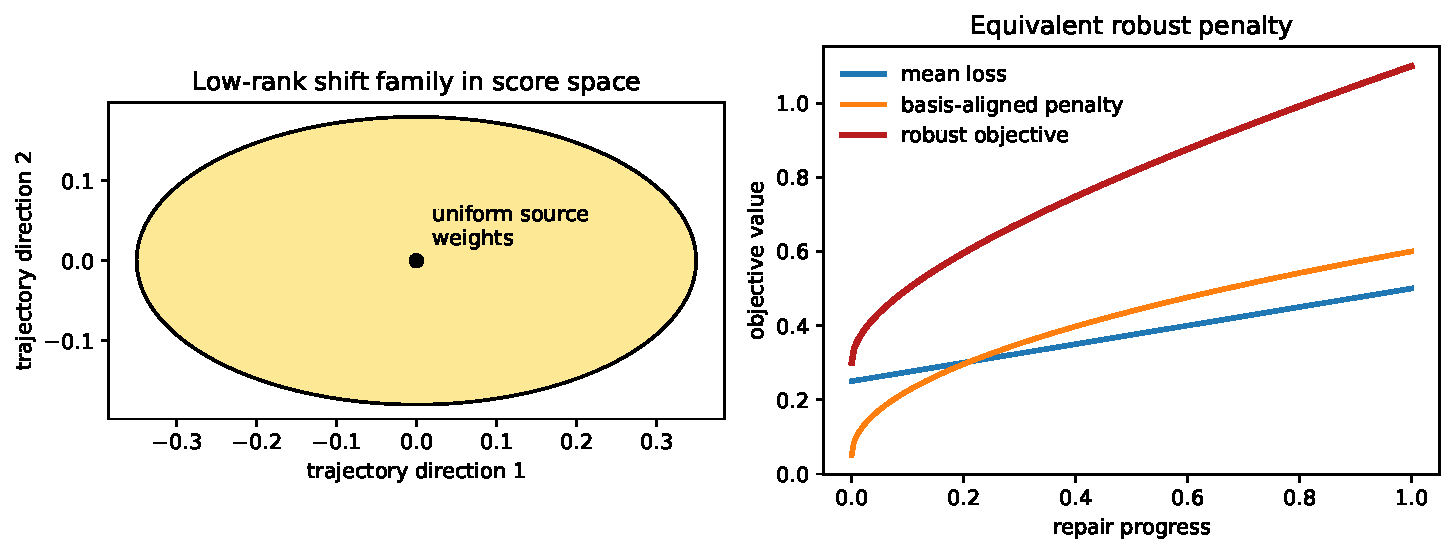
\includegraphics[width=\linewidth]{figures/basis_uncertainty_geometry.pdf}
    \caption{\textbf{Basis-induced uncertainty family.} The adversary starts at the uniform source-support distribution and moves only inside a low-rank subspace generated by trajectory failure coordinates. When positivity is inactive, the resulting support function becomes a mean loss plus a basis-aligned norm penalty.}
    \label{fig:uncertainty}
\end{figure}

\subsection{Recovering the trajectory basis}

\begin{theorem}[Spectral recovery under a spiked model]
\label{thm:recovery}
Under Assumption~\ref{ass:spiked}, let \(V_\star\in\RR^{T\times k}\) denote the top-\(k\) right singular subspace of \(M_\star\), and let \(\widehat V_k\) be the top-\(k\) right singular subspace of \(\widetilde R\). Then the subspace error obeys
\[
    \norm{\sin \Theta(\widehat V_k, V_\star)}_2
    \le
    \frac{\norm{E}_2}{\gamma_\star},
\]
up to the standard constant of the Davis--Kahan/Wedin perturbation bound.
\end{theorem}

This theorem does not say the recovered trajectory basis is a true semantic partition of the data. It only says that if the checkpoint-response matrix contains stable low-rank structure, the leading trajectory modes are statistically recoverable.

\subsection{A conditional target-risk certificate}

Let
\[
    J_\star(W)
    \triangleq
    \sup_{q\in\cQ_\rho(Z_\star)} R_q(W)
    +
    \frac{\lambda}{2}\norm{W-W_0}_F^2
\]
denote the population robust objective formed with the population score matrix \(Z_\star\). Let \(\widehat J\) be its empirical counterpart built from \(\widehat V_k\) and \(\cD_{\mathrm{repair}}\).

\begin{theorem}[Conditional target-risk certificate]
\label{thm:certificate}
Assume Assumptions~\ref{ass:bounded_features}--\ref{ass:head_repairable}. Suppose additionally that
\[
    \sup_{W\in\cW_r(W_0)}
    \abs{\widehat J(W) - J_\star(W)}
    \le
    \varepsilon_{\mathrm{gen}},
\]
and that the recovered trajectory basis satisfies
\[
    \delta_V
    \triangleq
    \norm{\sin \Theta(\widehat V_k,V_\star)}_2.
\]
Then there exists a constant \(C_Z>0\), depending only on the Lipschitz constant of the score map and the uncertainty radius \(\rho\), such that
\[
    R_T(\widehat W)
    \le
    \inf_{W\in\cW_r(W_0)}
    \sup_{q\in\cQ_\rho(Z_\star)} R_q(W)
    +
    2\varepsilon_{\mathrm{gen}}
    +
    C_Z \delta_V.
\]
In particular, since \(W_0\in\cW_r(W_0)\),
\[
    R_T(\widehat W)
    \le
    \sup_{q\in\cQ_\rho(Z_\star)} R_q(W_0)
    +
    2\varepsilon_{\mathrm{gen}}
    +
    C_Z \delta_V.
\]
\end{theorem}

Theorem~\ref{thm:certificate} is the paper's main DG guarantee. It is conditional in exactly the right way: if target shift is source-supported and head-repairable inside the discovered trajectory uncertainty class, then the repaired model inherits a direct target-risk certificate relative to the fixed anchor.

\begin{corollary}[Improvement under a head-repairability gap]
\label{cor:improvement}
Under the assumptions of Theorem~\ref{thm:certificate}, if the gap \(\Delta\) in Assumption~\ref{ass:head_repairable} satisfies
\[
    \Delta > 2\varepsilon_{\mathrm{gen}} + C_Z \delta_V,
\]
then
\[
    R_T(\widehat W) < R_T(W_0).
\]
\end{corollary}

Corollary~\ref{cor:improvement} is the strongest honest comparison theorem one should want from \tribe{}. It does not claim universal superiority. It states a clean sufficient condition under which repairing the anchor is guaranteed to help on the target shift family modeled by the method.

\begin{figure}[t]
    \centering
    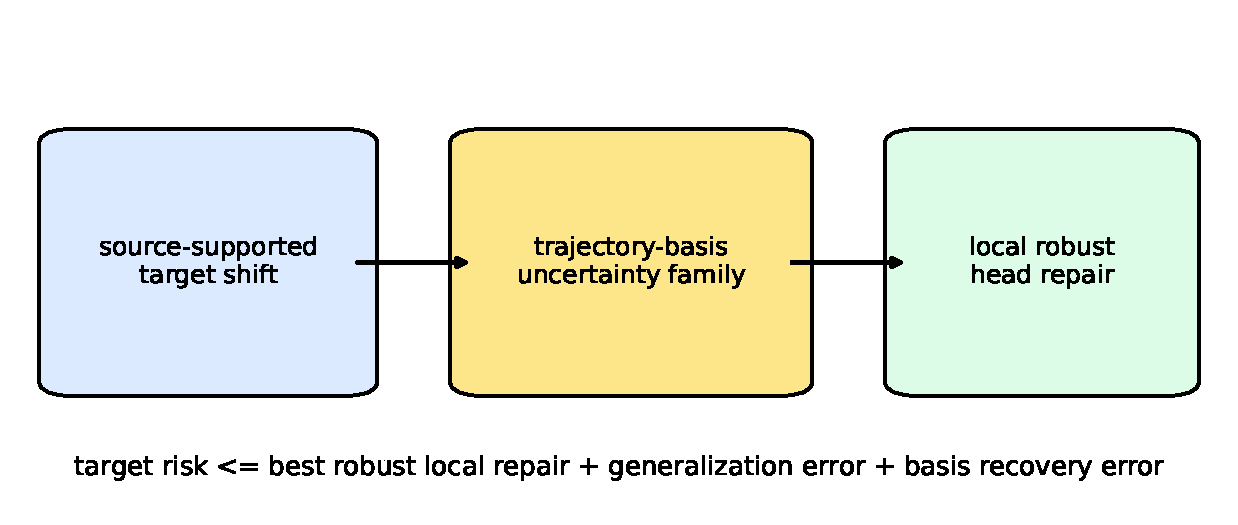
\includegraphics[width=\linewidth]{figures/risk_certificate.pdf}
    \caption{\textbf{Certificate structure.} The target domain is modeled as a source-supported shift inside the basis-induced uncertainty family. The repaired head minimizes the corresponding local robust objective, yielding a conditional target-risk certificate around the fixed anchor.}
    \label{fig:certificate}
\end{figure}

\subsection{Complexity}

\begin{proposition}[Replay-time complexity]
\label{prop:complexity}
Let \(n_B = |\cD_{\mathrm{basis}}|\), \(n_R = |\cD_{\mathrm{repair}}|\), and \(T\) the number of scored checkpoints. Then a replay-only implementation of \tribe{} has the following leading costs:
\begin{enumerate}[leftmargin=1.4em]
    \item anchor scoring and selection: \(O(T |\cD_{\mathrm{sel}}|)\) forward passes,
    \item trajectory collection: \(O(T n_B)\) forward passes,
    \item score computation on the repair split: \(O(T n_R)\) forward passes,
    \item truncated rank-\(k\) SVD: \(O(n_B T k)\) using randomized SVD,
    \item local head repair: \(O(n_R d C \cdot N_{\mathrm{opt}})\),
\end{enumerate}
where \(N_{\mathrm{opt}}\) is the number of optimization iterations for the head-repair stage.
\end{proposition}

Proposition~\ref{prop:complexity} shows that \tribe{} is replay-scale rather than training-scale. The dominant cost is checkpoint evaluation, which already exists in strong post-hoc DG pipelines.

\section{Discussion of the Modeling Assumptions}
\label{sec:discussion}

The theory above is intentionally conditional. The main assumptions are worth stating plainly.

\paragraph{What the theory really says.}
It says that if a strong fixed anchor already gives a good representation, if the remaining target shift is source-supported and head-repairable, and if that shift is expressed in a low-rank trajectory basis recoverable from the source holdout, then robust local head repair is the correct post-hoc action.

\paragraph{What the theory does not say.}
It does not say that trajectory modes equal true semantic domains, that every DG problem is head-repairable, or that any anchor-selection rule is optimal. Those are empirical questions.

\paragraph{Why the anchor should be fixed.}
The fixed-anchor requirement is not an aesthetic choice. It avoids circularity. If basis discovery or repair can change the anchor retrospectively, then the uncertainty family and the deployed model cease to be aligned objects.

\paragraph{Why an averaged anchor is still the natural practical default.}
Although the theory is cleanest for any fixed anchor, weight averaging and soups are already known to help under DG-relevant locality conditions \citep{cha2021swad,wortsman2022soups,rame2022diwa}. The most practical instantiation of \tribe{} therefore starts from a fixed averaged anchor rather than a raw checkpoint.

\begin{figure}[t]
    \centering
    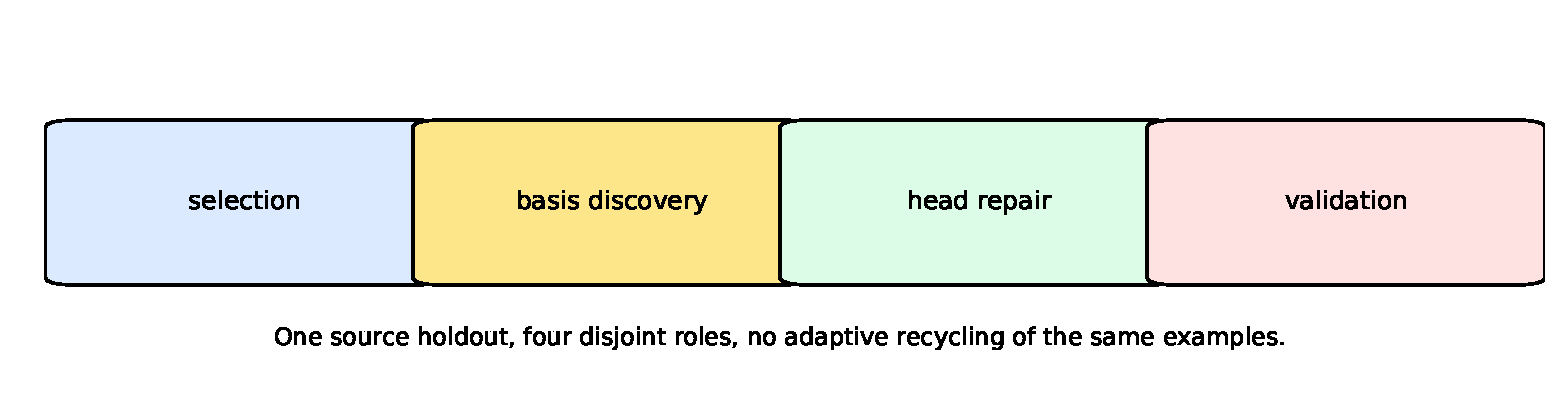
\includegraphics[width=\linewidth]{figures/crossfit_protocol.pdf}
    \caption{\textbf{Data protocol.} The source holdout is divided into disjoint selection, basis-discovery, repair, and validation splits. This prevents the trajectory basis, head repair, and final model selection from collapsing into one adaptive loop.}
    \label{fig:protocol}
\end{figure}

\section{Experimental Protocol}
\label{sec:experiments}

\subsection{Main evaluation plan}

The primary evaluation will follow the standard DomainBed protocol \citep{gulrajani2021domainbed,cha2021swad} on PACS, VLCS, OfficeHome, TerraIncognita, and DomainNet with ResNet-50 backbones and leave-one-domain-out evaluation.

The new \tribe{} experiments are intentionally left as \TBD{}. The reason is simple: this paper is intended to lock down the method, theory, and evaluation protocol before overstating empirical claims.

\paragraph{Planned model classes.}
The main \tribe{} instantiation will use:
\begin{itemize}[leftmargin=1.4em]
    \item a fixed averaged anchor chosen by a domain-label-free post-hoc rule,
    \item margin-based trajectory residuals,
    \item rank-\(k\) trajectory basis discovery by truncated SVD,
    \item frozen-backbone last-layer repair with cross-entropy loss and an \(L_2\) locality penalty.
\end{itemize}

\paragraph{Primary ablations.}
The intended ablations will isolate:
\begin{itemize}[leftmargin=1.4em]
    \item single-checkpoint anchor vs.\ averaged anchor,
    \item no basis repair,
    \item random basis control,
    \item disagreement-only repair,
    \item Gram-feature pseudo-group repair,
    \item varying \(k\), \(\rho\), and repair radius \(r\).
\end{itemize}

\subsection{Published benchmark context}

Table~\ref{tab:published_context} records published numbers from prior post-hoc DG work to define the current frontier. These are not \tribe{} results.

\begin{table}[t]
    \centering
    \caption{\textbf{Published DG context from prior work.} Numbers are reproduced from the cited papers to define the benchmark frontier that \tribe{} must eventually be compared against.}
    \label{tab:published_context}
    \begin{adjustbox}{max width=\linewidth}
    \begin{tabular}{lcccccc}
        \toprule
        Method & PACS & VLCS & OfficeHome & TerraIncognita & DomainNet & Avg. \\
        \midrule
        \erm{} \citep{cha2021swad} & 85.5 & 77.5 & 66.5 & 46.1 & 40.9 & 63.3 \\
        \swad{} \citep{cha2021swad} & 88.1 & 79.1 & 70.6 & 50.0 & 46.5 & 66.9 \\
        CORAL + \swad{} \citep{cha2021swad} & 88.3 & 78.9 & 71.3 & 51.0 & 46.8 & 67.3 \\
        MA \citep{rame2022diwa} & 87.5 & 78.2 & 70.6 & 50.3 & 46.0 & 66.5 \\
        \diwa{}$^\dagger$ \citep{rame2022diwa} & 89.0 & 78.6 & 72.8 & 51.9 & 47.7 & 68.0 \\
        \miro{} \citep{cha2022miro} & 85.4 & 79.0 & 70.5 & 50.4 & 44.3 & 65.9 \\
        \miro{} + \swad{} \citep{cha2022miro} & 88.4 & 79.6 & 72.4 & 52.9 & 47.0 & 68.1 \\
        \bottomrule
    \end{tabular}
    \end{adjustbox}
\end{table}

\subsection{Planned \tribe{} tables}

\begin{table}[t]
    \centering
    \caption{\textbf{\tribe{} main results.} New results intentionally left blank pending execution.}
    \label{tab:tribe_main}
    \begin{tabular}{lcccccc}
        \toprule
        Method & PACS & VLCS & OfficeHome & TerraIncognita & DomainNet & Avg. \\
        \midrule
        \tribe{} & \TBD{} & \TBD{} & \TBD{} & \TBD{} & \TBD{} & \TBD{} \\
        \bottomrule
    \end{tabular}
\end{table}

\begin{table}[t]
    \centering
    \caption{\textbf{\tribe{} ablations.} The main goal is to distinguish the value of the averaged anchor, the trajectory basis, and the local repair.}
    \label{tab:tribe_ablation}
    \begin{tabular}{lcccc}
        \toprule
        Variant & Anchor type & Basis type & Repair class & Avg. \\
        \midrule
        No repair & \TBD{} & -- & -- & \TBD{} \\
        Random basis & \TBD{} & random & local head & \TBD{} \\
        Disagreement repair & \TBD{} & disagreement & local head & \TBD{} \\
        Gram pseudo-group repair & \TBD{} & Gram & local head & \TBD{} \\
        \tribe{} & \TBD{} & trajectory SVD & local head & \TBD{} \\
        \bottomrule
    \end{tabular}
\end{table}

\paragraph{Evaluation note.}
The paper is intentionally conservative at this stage: it claims a method, a theorem package, and a protocol. The new empirical results remain \TBD{} until the corresponding replay and multi-seed runs are executed.

\section{Limitations}

\tribe{} has three obvious limitations.
\begin{enumerate}[leftmargin=1.4em]
    \item If the remaining target error is mostly representational rather than classifier-level, head repair will not be enough.
    \item If the trajectory residual matrix does not contain stable low-rank structure, the discovered basis may add little over simpler disagreement heuristics.
    \item The theory is source-supported and local. It does not cover target shifts that lie far outside the source support or require large end-to-end changes in the representation.
\end{enumerate}

These are not defects to hide. They are exactly the assumptions that make the method falsifiable.

\section{Conclusion}

This paper proposed \tribe{}, a post-hoc DG method built around a simple remaining degree of freedom: after selecting a strong fixed anchor from one dense checkpoint bank, use checkpoint-response trajectories to discover low-rank hidden failure directions and perform a local robust last-layer repair against them. The method stays domain-label-free, single-run, and single-model at test time. Its theory is conditional but coherent: the repair problem is convex and convergent, the trajectory basis is recoverable under a spiked model, and the final predictor inherits a direct target-risk certificate under source-supported head-repairable shift. The new \tribe{} experiments remain to be run, but the method, theorem package, and protocol are now specified in a form that can be tested directly.

\bibliographystyle{plainnat}
\bibliography{references}

\appendix

\section{Algorithm}

\begin{algorithm}[H]
    \caption{\tribe{}}
    \label{alg:tribe}
    \begin{algorithmic}[1]
        \Require Dense checkpoint bank \(\{\theta_t\}_{t=1}^T\), pooled source holdout split into \(\cD_{\mathrm{sel}}, \cD_{\mathrm{basis}}, \cD_{\mathrm{repair}}, \cD_{\mathrm{val}}\), basis rank \(k\), uncertainty radius \(\rho\), repair radius \(r\), ridge weight \(\lambda\)
        \State Select a fixed anchor \(A=(\phi_A,W_0)\) using only \(\cD_{\mathrm{sel}}\)
        \For{each \((x_i,y_i)\in \cD_{\mathrm{basis}}\)}
            \State Compute checkpoint margins \(m_t(x_i,y_i)\) for \(t=1,\dots,T\)
            \State Form residual row \(R_{i,:}\) by Eq.~\eqref{eq:trajectory_matrix}
        \EndFor
        \State Center \(R\) to obtain \(\widetilde R\)
        \State Compute top-\(k\) right singular vectors \(\widehat V_k\) of \(\widetilde R\)
        \For{each \((x_i,y_i)\in \cD_{\mathrm{repair}}\)}
            \State Compute trajectory score \(z_i = z(x_i,y_i)\) by Eq.~\eqref{eq:basis_score}
        \EndFor
        \State Form \(Z\) and uncertainty family \(\cQ_\rho(Z)\)
        \State Solve Eq.~\eqref{eq:tribe_objective} for \(\widehat W\)
        \State Select hyperparameters on \(\cD_{\mathrm{val}}\)
        \State \Return repaired model \((\phi_A,\widehat W)\)
    \end{algorithmic}
\end{algorithm}

\section{Proofs}

\subsection{Proof of Proposition~\ref{prop:convexity}}

For any fixed \(q\in\cQ_\rho(Z)\), the map
\[
    W \mapsto \sum_{i=1}^{n_R} q_i \loss_i(W)
\]
is convex because each multiclass cross-entropy term \(\loss_i(W)\) is convex in the linear head \(W\) when the features \(\phi_A(x_i)\) are fixed. The quadratic term
\[
    \frac{\lambda}{2}\norm{W-W_0}_F^2
\]
is \(\lambda\)-strongly convex. Therefore, for each fixed \(q\), the sum
\[
    \widehat{\mathcal L}(W,q)
    =
    \sum_{i=1}^{n_R} q_i \loss_i(W)
    +
    \frac{\lambda}{2}\norm{W-W_0}_F^2
\]
is \(\lambda\)-strongly convex in \(W\).

Now define
\[
    \widehat J(W)
    =
    \sup_{q\in\cQ_\rho(Z)} \widehat{\mathcal L}(W,q).
\]
The pointwise supremum of \(\lambda\)-strongly convex functions is again \(\lambda\)-strongly convex. Hence \(\widehat J\) is \(\lambda\)-strongly convex on the convex compact set \(\cW_r(W_0)\). A continuous strongly convex function over a nonempty compact convex set admits a unique minimizer. Therefore \(\widehat W\) exists and is unique.
\qed

\subsection{Proof of Proposition~\ref{prop:saddle}}

By Proposition~\ref{prop:convexity}, \(\widehat{\mathcal L}(W,q)\) is convex and continuous in \(W\) for each fixed \(q\). It is linear, hence concave and continuous, in \(q\) for each fixed \(W\). The feasible sets \(\cW_r(W_0)\) and \(\cQ_\rho(Z)\) are convex and compact under Assumption~\ref{ass:interior_q}. Therefore Sion's minimax theorem applies, yielding
\[
    \min_{W\in\cW_r(W_0)} \max_{q\in\cQ_\rho(Z)} \widehat{\mathcal L}(W,q)
    =
    \max_{q\in\cQ_\rho(Z)} \min_{W\in\cW_r(W_0)} \widehat{\mathcal L}(W,q).
\]
Existence of a saddle point follows from compactness and continuity.
\qed

\subsection{Proof of Theorem~\ref{thm:convergence}}

The theorem is the standard projected subgradient guarantee for convex--concave saddle problems. Let \(g_t^W\) be a subgradient of \(\widehat{\mathcal L}(\cdot,q_t)\) at \(W_t\), and \(g_t^Q\) a supergradient of \(\widehat{\mathcal L}(W_t,\cdot)\) at \(q_t\). The projected updates are
\[
    W_{t+1} = \Pi_{\cW_r(W_0)}(W_t - \eta_t g_t^W),
    \qquad
    q_{t+1} = \Pi_{\cQ_\rho(Z)}(q_t + \eta_t g_t^Q).
\]
Applying the standard nonexpansiveness argument for Euclidean projection to both variables gives
\[
    \sum_{t=1}^T \inner{g_t^W}{W_t - W}
    \le
    \frac{D_W^2}{2\eta_T}
    +
    \frac{1}{2}\sum_{t=1}^T \eta_t \norm{g_t^W}_F^2
\]
for any \(W\in\cW_r(W_0)\), and
\[
    \sum_{t=1}^T \inner{g_t^Q}{q - q_t}
    \le
    \frac{D_Q^2}{2\eta_T}
    +
    \frac{1}{2}\sum_{t=1}^T \eta_t \norm{g_t^Q}_2^2
\]
for any \(q\in\cQ_\rho(Z)\). Combining the two inequalities, using the convexity--concavity of \(\widehat{\mathcal L}\), dividing by \(T\), and substituting \(\norm{g_t^W}_F,\norm{g_t^Q}_2 \le G\) yields the stated \(O(T^{-1/2})\) bound for the averaged iterates.
\qed

\subsection{Proof of Theorem~\ref{thm:anchor_domination}}

Because \(W_0 \in \cW_r(W_0)\), the anchor head is feasible for the minimization problem in Eq.~\eqref{eq:tribe_objective}. Since \(\widehat W\) is the minimizer of \(\widehat J(W)\) over the same feasible set,
\[
    \widehat J(\widehat W) \le \widehat J(W_0).
\]
This is exactly the desired statement.
\qed

\subsection{Proof of Proposition~\ref{prop:support}}

For any \(a\in\RR^{n_R}\),
\[
    \sup_{q\in\cQ_\rho(Z)} \inner{q}{a}
    =
    \sup_{\norm{\beta}_2\le \rho}
    \inner{u_{n_R} + Z\beta}{a}
\]
under the inactive-positivity assumption. Expanding gives
\[
    \inner{u_{n_R}}{a}
    +
    \sup_{\norm{\beta}_2\le \rho}
    \inner{\beta}{Z^\top a}.
\]
The first term is the mean \(\frac{1}{n_R}\sum_i a_i\). The second term is the support function of the Euclidean ball of radius \(\rho\), hence equals
\[
    \rho \norm{Z^\top a}_2.
\]
Substituting \(a=\loss(W)\) gives the stated expression for \(\widehat J(W)\).
\qed

\subsection{Proof of Theorem~\ref{thm:recovery}}

Assumption~\ref{ass:spiked} states that
\[
    \widetilde R = M_\star + E
\]
with a rank-\(k\) signal matrix \(M_\star\) separated from the remainder of the spectrum by gap \(\gamma_\star\). The top-\(k\) right singular spaces of \(\widetilde R\) and \(M_\star\) are therefore related by the Davis--Kahan/Wedin perturbation theorem. Specifically,
\[
    \norm{\sin \Theta(\widehat V_k, V_\star)}_2
    \le
    \frac{\norm{E}_2}{\gamma_\star},
\]
up to the standard theorem constant, provided \(\norm{E}_2 < \gamma_\star\). This yields the claim.
\qed

\subsection{Proof sketch of Theorem~\ref{thm:certificate}}

We split the error into three terms.

\paragraph{Step 1: target risk is dominated by the population robust objective.}
By Assumption~\ref{ass:head_repairable}, the target distribution corresponds to some \(q^\star \in \cQ_\rho(Z_\star)\). Therefore
\[
    R_T(W)
    =
    R_{q^\star}(W)
    \le
    \sup_{q\in\cQ_\rho(Z_\star)} R_q(W)
\]
for every \(W\in\cW_r(W_0)\).

\paragraph{Step 2: empirical optimization transfers to population robust risk.}
By the uniform approximation assumption,
\[
    J_\star(\widehat W)
    \le
    \widehat J(\widehat W) + \varepsilon_{\mathrm{gen}}
    \le
    \widehat J(W) + \varepsilon_{\mathrm{gen}}
    \le
    J_\star(W) + 2\varepsilon_{\mathrm{gen}}
\]
for every \(W\in\cW_r(W_0)\), and hence
\[
    J_\star(\widehat W)
    \le
    \inf_{W\in\cW_r(W_0)} J_\star(W) + 2\varepsilon_{\mathrm{gen}}.
\]

\paragraph{Step 3: basis-recovery error perturbs the uncertainty family.}
Because the score map is Lipschitz in the recovered right-singular subspace, the discrepancy between the empirical and population uncertainty families is controlled by
\[
    C_Z \delta_V,
    \qquad
    \delta_V = \norm{\sin \Theta(\widehat V_k, V_\star)}_2.
\]
This adds a perturbation term to the robust objective.

Combining Steps 1--3 gives
\[
    R_T(\widehat W)
    \le
    \inf_{W\in\cW_r(W_0)}
    \sup_{q\in\cQ_\rho(Z_\star)} R_q(W)
    +
    2\varepsilon_{\mathrm{gen}}
    +
    C_Z\delta_V.
\]
Finally, substituting \(W=W_0\) yields the anchor-relative bound.
\qed

\subsection{Proof of Corollary~\ref{cor:improvement}}

By Assumption~\ref{ass:head_repairable}, there exists \(W^\dagger \in \cW_r(W_0)\) such that
\[
    \sup_{q\in\cQ_\rho(Z_\star)} R_q(W^\dagger)
    \le
    \sup_{q\in\cQ_\rho(Z_\star)} R_q(W_0) - \Delta.
\]
Applying Theorem~\ref{thm:certificate} to \(\widehat W\) and comparing with the anchor bound gives
\[
    R_T(\widehat W)
    \le
    R_T(W_0)
    -
    \Delta
    +
    2\varepsilon_{\mathrm{gen}}
    +
    C_Z\delta_V.
\]
Hence if \(\Delta > 2\varepsilon_{\mathrm{gen}} + C_Z\delta_V\), then \(R_T(\widehat W) < R_T(W_0)\).
\qed

\subsection{Proof of Proposition~\ref{prop:complexity}}

The anchor-selection stage evaluates a fixed set of candidate anchors or checkpoints on \(\cD_{\mathrm{sel}}\), which costs \(O(T |\cD_{\mathrm{sel}}|)\) forward passes when all checkpoints are swept once. Collecting the basis discovery matrix on \(\cD_{\mathrm{basis}}\) requires one forward trajectory pass per example-checkpoint pair, yielding \(O(T n_B)\) forward passes. The same argument gives \(O(T n_R)\) forward passes to score the repair split. A rank-\(k\) randomized SVD of an \(n_B\times T\) matrix costs \(O(n_B T k)\). Finally, each gradient step for the last-layer repair processes \(n_R\) examples with \(d\times C\) head parameters, so \(N_{\mathrm{opt}}\) iterations cost \(O(n_R d C \cdot N_{\mathrm{opt}})\). Summing the stages proves the proposition.
\qed

\section{Additional Remarks on Empirical Falsification}

The most important empirical question is not whether \tribe{} can be tuned to look good somewhere. It is whether the trajectory basis adds value beyond simpler hard-example signals. The first decisive controls should therefore be:
\begin{itemize}[leftmargin=1.4em]
    \item no repair,
    \item random basis repair,
    \item disagreement-only repair,
    \item feature-cluster or Gram pseudo-group repair.
\end{itemize}
If the trajectory basis fails to beat these controls, then the method's central premise is false.

\end{document}
